\chapter[The End - A Reflection on the Past, the Present, and the Future]{The End - A Reflection on the Past, the Present, and the Future}\label{chap:the_end}

\section{Future Work}

-- see ``ten recommendations'' in ema's diss
-- be frank and say we don't want to create ``recommendations'' or ``guidelines'', because it takes years and more diverse samples to solidify such. Therefore, we think it's better to show ``ideas'' what this can mean and where the topic is going. 

\todo{relate each idea to the PST!}

\subsection{Personalizing Password Policies}\label{sec:pst:personalizing-policies}

Segreti \etal SOUPS 2017
\cite{Seitz2017PPT}
\cite{Segreti2017AdaptivePolicies}

\subsection{Keystrokes as Reuse Heuristics}
Reuse is the worst. We should design a persuasive strategy that shows alternatives to reused passwords. As a first step, we need to detect that the password a user just entered has been reused on other websites. Since this is not bad per se, we also need to check how strong it is, and how likey it is a ``throw away'' password that users don't care about anyway. -- elaborate on this. Show an updated flow chart from CHI EA 


\subsection{Contextualizing Password Feedback}
like \cite{Kroeze2012GamifyingAuthentication} Pokémon Go could use an evolving Pokemon as password strength feedback. 

``wuerstel meter'' as an example that we implemented.

minimizes habituation effects as mentioned by Ur \etal \cite{Ur2012HelpingUsersCreateBetterPasswords}.

\subsection{What do other people do? Clichés and biased views of password selection strategies}
people are biased to think that their password strategy is unique, i.e. they do not realize that other users behave similarly. it would be interesting to study the revelation process - ask people on the street how they think that others create their passwords for different categories. independent variables: who creates a password, for what context?

social patterns helpful: Instead of saying a password is better than 90\% of other \textit{users} we could frame it as ``this password lowers your chance of being attacked by XX percent'' or ``this password is better than 90\% of passwords used on the internet''. issues: it's kind of hard to really be truthful here. deceptive in some ways and that's not something we want. 

\subsection{Post 3rd Party Breach Password Invalidation}
if a data leak is made public, sites can use the leaked passwords to audit the users on their sites. if they find that passwords have been compromised, they should decide (depending on a matching user name) if the password on their site should be invalidated and the user prompted to update it.

kind of resembles a post-hoc blacklist.  

catch: carefully craft Password Reset Emails \cite{Kim2017TooBusy}

risks: users could be confused, looks like a phishing attack (why was my account hacked?)

feature for password meters to determine stringency: 
there could be a framework that uses \url{https://haveibeenpwned.com/API/v2} to adjust stringency 

from \cite{Bishop1995ProactivePasswordChecking}: ``Many sites have responded to this threat with a reactive solution -- they scan their own password files and advise those users whose passwords they are able to crack. The problem with this solution is that while the local site is testing its security, the password file is still vulnerable from the outside. The other problems, of course, are that the testing is very time-consuming and only reports on those passwords it is able to crack. It does nothing to address user passwords which fall outside of the specific test cases (e.g., it is possible for a user to use as a password the letters ``query'' if this combination is not in the in-house test dictionary, it will not be detected, but there is nothing to stop an outside cracker from having a more sophisticated dictionary!).''

\subsection{Helping to Make Sense of a Breach}
how does user behavior change after a breach? not much says Huh \etal \cite{Huh2017TooBusy}. But it would be interesting to correlate other factors with altered behavior: do different personality traits influence how a user ``cleans up the mess'' after a breach?


\section{Final Thoughts}
Lorem Epson. 

\begin{figure}[htpb]
	\centering
	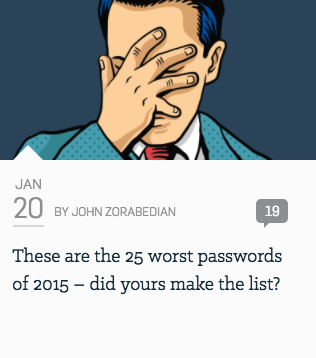
\includegraphics[width=0.3\linewidth]{shaming/nakedsecurity-sophos}
	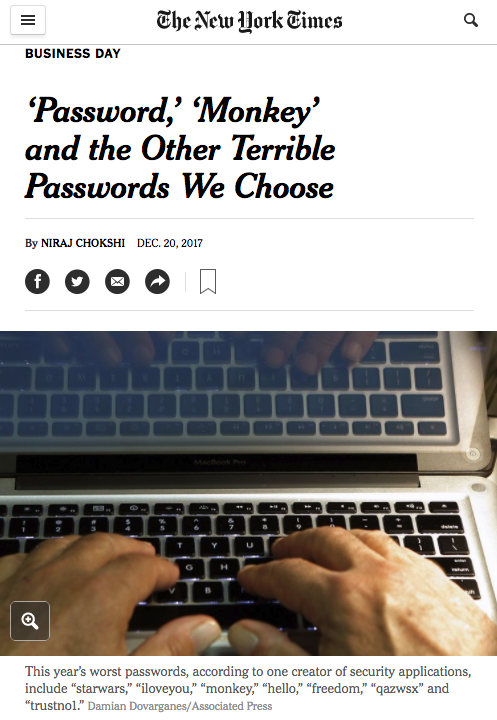
\includegraphics[width=0.3\linewidth]{shaming/nytimes}
	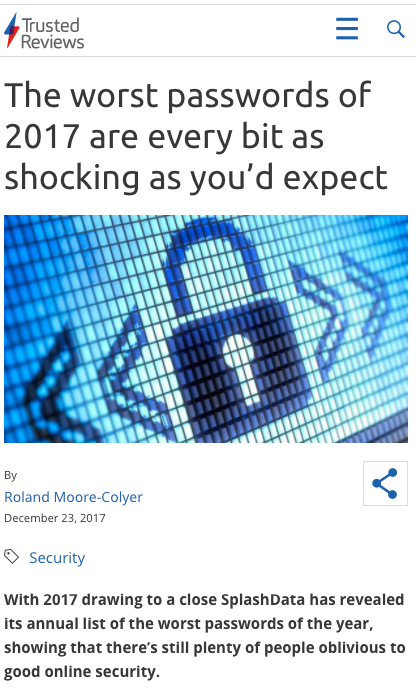
\includegraphics[width=0.3\linewidth]{shaming/trusted-reviews}
\end{figure}

Key thoughts

\begin{itemize}
\item Passwords are bad. Let's hope passwords vanish at some point. Make machines intelligent enough to decide if a user should be granted access or not. But this brings new problems.
\item Maybe passwords are the vinyl records of usable security - everyone agrees that it's kind of an obsolete technology but there's something to it that ensure they don't disappear. %TODO come up with a better analogy.
 \item  if passwords become obsolete tomorrow, many of us will not grief. 
 \item  the media should stop shaming the users 
 \item  it's okay to forget passwords! reference to the article Franziska shared with me (SZ,  01.12.2017 ``Die Kunst zu vergessen'' \footurl{http://www.sueddeutsche.de/wissen/neurowissenschaft-die-kunst-zu-vergessen-1.3772438}{02.01.2018}.)
 \item 	ad networks for webpages can undermine any attempt to secure one's account. Too many websites show ads that can run harmful scripts. yes, adblockers do prevent this, but not everyone has one installed (especially novice users don't). Frightening research on this: \footurl{https://freedom-to-tinker.com/2017/12/27/no-boundaries-for-user-identities-web-trackers-exploit-browser-login-managers/}{02.01.2018}
\end{itemize}

It's interesting that often the same idea pops up every other year. so although there are no replication studies, evaluating the same idea multiple times with different setups and specifics, kind of goes in that direction. 


%TODO I have more thann 100 ``takeaways'' from papers. This could be a funny ``sermon'' too (Luther's 100 theses);